%% This is file `elsarticle-template-1-num.tex',
%% %% Copyright 2009 Elsevier Ltd
%%
%% This file is part of the 'Elsarticle Bundle'.
%% ---------------------------------------------
%%
%% It may be distributed under the conditions of the LaTeX Project Public
%% License, either version 1.2 of this license or (at your option) any
%% later version.  The latest version of this license is in
%%    http://www.latex-project.org/lppl.txt
%% and version 1.2 or later is part of all distributions of LaTeX
%% version 1999/12/01 or later.
%%
%% The list of all files belonging to the 'Elsarticle Bundle' is
%% given in the file `manifest.txt'.
%%
%% Template article for Elsevier's document class `elsarticle'
%% with numbered style bibliographic references
%%
%% $Id: elsarticle-template-1-num.tex 149 2009-10-08 05:01:15Z rishi $
%% $URL: http://lenova.river-valley.com/svn/elsbst/trunk/elsarticle-template-1-num.tex $
%%

%\documentclass[]{article} %\documentclass[final,3p,12pt]{elsarticle}
%\documentclass[final,12pt,times]{elsarticle}

%% Use the option review to obtain double line spacing
\documentclass[preprint,review,12pt]{elsarticle}

%% Use the options 1p,twocolumn; 3p; 3p,twocolumn; 5p; or 5p,twocolumn
%% for a journal layout:
%% \documentclass[final,1p,times]{elsarticle}
%% \documentclass[final,1p,times,twocolumn]{elsarticle}
%% \documentclass[final,3p,times]{elsarticle}
%% \documentclass[final,3p,times,twocolumn]{elsarticle}
%% \documentclass[final,5p,times]{elsarticle}
%% \documentclass[final,5p,times,twocolumn]{elsarticle}

\usepackage{amssymb}
\usepackage{wrapfig}
\usepackage{lipsum}
\usepackage{natbib}

\usepackage{tikz}
\usetikzlibrary{shapes, arrows}

\tikzstyle{notary} = [rectangle, draw, text centered, text width=4em, fill=blue!20, minimum height=2em]
\tikzstyle{user}   = [rectangle, draw, text centered, text width=4em, fill=green!20, minimum height=2em]
\tikzstyle{server} = [rectangle, draw, text centered, text width=4em, fill=red!20, minimum height=2em]
\tikzstyle{single}   = [draw, -latex']
\tikzstyle{double}   = [draw, latex-latex']

% http://tex.stackexchange.com/questions/35712/modify-footer-used-by-elsarticle-cls
\makeatletter
\def\ps@pprintTitle{
    \let\@oddhead\@empty
    \let\@evenhead\@empty
    \def\@oddfoot{\centerline{\thepage}}
    \let\@evenfoot\@oddfoot}
\makeatother

\journal{University of Guelph; CIS*4110}

\begin{document}

\begin{frontmatter}

\title{Improving Perspectives by adding functionally to update record of SSL certificates upon request}

\author[doug]{Douglas Anderson}
\author[eric]{Eric Boyd}
\author[james]{James Kelly}
\address[doug]{dander01@uoguelph.ca}
\address[eric]{boyde@uoguelph.ca}
\address[james]{kellyj@uoguelph.ca}


\begin{abstract}

Today's web is secured with SSL and TLS, which utilizes RSA to create secure
connections between servers and users. To ensure that the users are
communicating with the web server they intend and not someone masquerading as
the server, Certificate Authorities (CAs) are considered to be secure trusted
parties that can confirm the identity of the server. While better than a 
completely insecure protocol, CAs can be compromised with Man-in-the-Middle
(MitM) attacks and leave users vulnerable. In an effort to fix this
weaknesses in the CA, The Perspectives Project uses a
constellation of notary servers spread out across the Internet to monitor the
SSL certificate signatures over time. Users install a Firefox extension that
compares the signature of the certificate given to them from the server to the
certificates observed by the notaries. Our augmentation to the Perspectives
system allows web servers currently being monitored by a number of notaries to
send a message to each of these notaries when the server changes their SSL 
certificate. This mitigates the lag between the certificate change and 
observation and therefore protects the users more efficeiently.

\end{abstract}

\begin{keyword}
% keywords here, in the form: keyword \sep keyword
Security \sep
SSL \sep
Certificate Authorities \sep
Perspectives
\end{keyword}

\end{frontmatter}

\section{Introduction}
\label{intro}

In the modern world the Internet holds a very important role in commerce and
social aspects of life and both of these pursuits require the ability for two or
more parties to communicate securely. To facilitate this secure communication,
the Internet has resorted to using the SSL (Secure Socket Layer) and it
successor TLS (Transport Security Layer) to protect the data being exchanged.
These protocols utilize public-private key pairs to facilitate RSA encryption.
While this protocol has been extremely successful it must rely on a Certificate Authority (CA) to
confirm the identity of the owner of public keys. While it is possible to
create `self-signed' certificates, browsers will warn users if a site uses one
of these certificate since it is impossible to verify who created the
certificate. 

Certificate Authorities are points in a network that issues and manages
security credentials and public keys for message encryption. CAs have been 
compromised in the past resulting in successful impersonations
of several popular, high profile websites.  In 2011 the central authority
Comodo Group, Inc. was hacked. The attack was easily executed
because of Comodo's extremely weak password system that was easily broken with a word
list. The hacker made off with the SSL certificates for various sites including 
Gmail, Yahoo Mail, Hotmail.  \citep{comodohack}
This allowed the hacker to perform Man-in-the-Middle (MitM) attacks on these sites by
impersonation the CAs for the various websites. It allowed the hacker to trick the site
user's computers into believing the fake SSL certificates were genuine and the hacker was
then able to read the site user's emails.  This illustrates the vulnerability
in the SSL protocol that central authorities create.

This vulnerability is what the Perspectives Project sets out to fix. Their
solution to removing central authorities is to create trusted services known as
notaries. These notaries work in tandem with a browser extension that allows the
user of the extension to select which of the notaries they would like to
trust. The system works by checking the SSL certificate signature the user is
given from the server against the SSL certificate signatures that the user's
trusted notaries have in their databases. If there is a discrepancy between the
certificate signature that the server has returned and the signatures that the
notaries have on record, the SSL connection is aborted.

\begin{figure}[h]
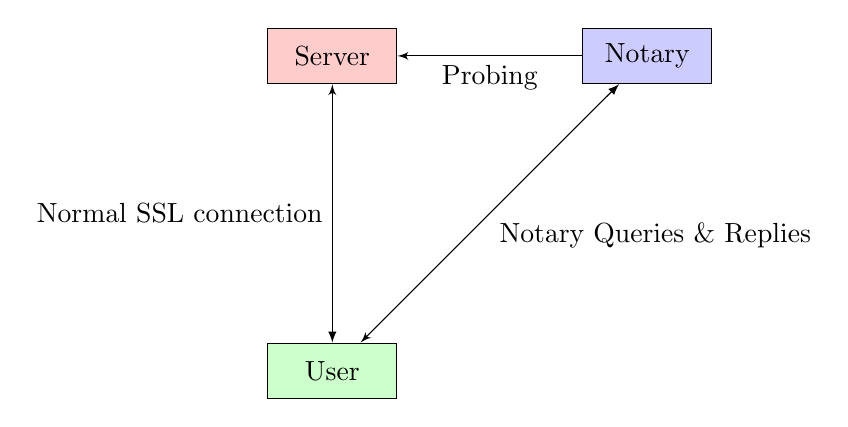
\begin{tikzpicture}[node distance = 4cm, auto]
    \node[server](server){Server};
    \node[notary, right of=server](note){Notary};
    \node[user, below of=server](user){User};
    \path[double](note) -- node {Notary Queries \& Replies}(user);
    \path[double](user) -- node {Normal SSL connection}(server);
    \path[single](note) -- node {Probing}(server);
\end{tikzpicture}
\caption{Normal Performance of the perspectives system.}
\end{figure}

\section{Method}
\label{Method}

For our project we attempted to build upon the Perspective Project by allowing
servers to send messages to notaries requesting that each notary acknowledge
the change of the SSL certificate. This fixes the problem in the Perspectives
Project that can occur when a server changes its SSL certificate and a user
queries the notary for that server's SSL certificate. Because the notary has
not yet updated its record of the SSL certificate the notery reports to the user that
there is a mismatch which may lead the user to abort their attempt to create an
SSL connection.

To send message requests to any notary, a server must first know if the notary exists. 
Since the notary presents itself as a normal user of the site when
it's probing, the server can not distinguish which of the users it must send a
probe request. Because of the short timeframe we had to work within, we hard-coded 
the address of the notary that the server would inform when its SSL certificate changes.

\begin{figure}[h]
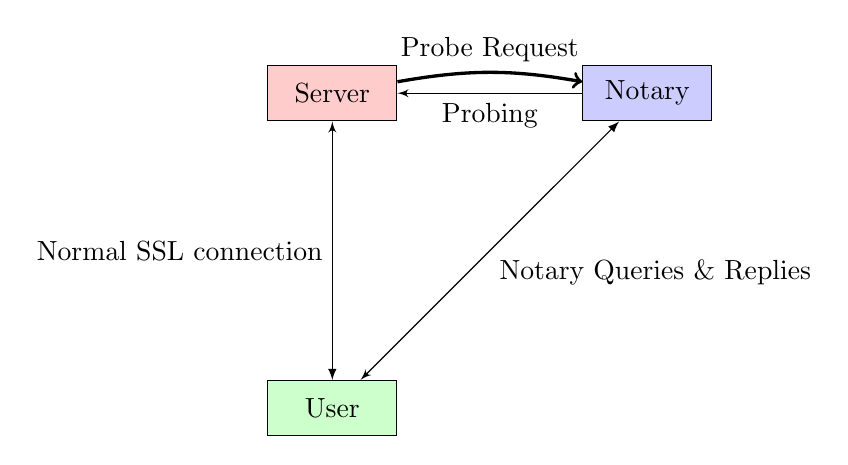
\begin{tikzpicture}[node distance = 4cm, auto]
    \node[server](server){Server};
    \node[notary, right of=server](note){Notary};
    \node[user, below of=server](user){User};
    \path[double](note) -- node {Notary Queries \& Replies}(user);
    \path[double](user) -- node {Normal SSL connection}(server);
    \path[single](note) -- node {Probing}(server);
    \path[->](server) edge[very thick, bend left=10] node{Probe Request}(note);
\end{tikzpicture}
\caption{Our modified perspective notary allows for the server to request that
    it's SSL certificate be probed and updated in the Notaries Database.}
\end{figure}

\section{Results}
\label{results}

\section{Conclusion}
\label{conclusion}

\section{Further Work}
\label{further work}

\subsection{Have notaries identify themselves to servers}

It would be very beneficial for notaries be able to inform servers that they
Perspectives notaries. This would allow servers to keep track of notaries
that have a record of them in their database so that when they do make a
change to their SSL certificate they can strive that inform all of the
notaries that have their old certificate so that it can be updated.

\subsection{Add preventive measures against DOS}

Since it is relatively computationally expensive for the notary to probe a
server for a SSL certificate signature it is possible to use these requests to
make a particular notary unresponsive to user queries. This could allow an
attacker to perform a man in the middle attack by rendering all of a users
notaries unresponsive before beginning their attack. While it may be possible
to prevent this attack on the part of the user by not continuing with the SSL
connection when none of their trusted notaries respond, This would still be
undesirable since it would prevent the user from making any secure connections.

\begin{enumerate}
    \item {Only probe a server when the probe request comes from the server itself}

        By only probing a server when the request comes from the server itself
        the possibility of external abuse is extremely limited. This method may
        be hard to implement in practise because it is possible for the
        attackers to spoof the origin of probe request to be the IP of the
        server.

    \item {Rate limit probe requests}

        By only allowing a certain number of probe requests in a period of time
        the notary can ensure that it does not compromise it's ability to
        respond to user request. This a common DOS prevention technique because
        of how effective it is, however it is possible that this method would
        become swamped at certain times since many websites change their SSL
        certificate at times of low traffic (e.g. 3AM).

\end{enumerate}

\section{References}
\label{references}
\nocite{*}
\bibliographystyle{plainnat}
\bibliography{report}

\end{document}

